\documentclass[a4paper]{article}
\usepackage{subfig}
\usepackage{algorithmicx}
\usepackage{algpseudocode}
\usepackage{graphicx}
\usepackage{vmargin}
\usepackage{mdwlist}
\setpapersize{A4}
\setmargins{2.5cm}       % margen izquierdo
{1.5cm}                        % margen superior
{16.5cm}                      % anchura del texto
{23.42cm}                    % altura del texto
{10pt}                           % altura de los encabezados
{1cm}                           % espacio entre el texto y los encabezados
{0pt}                             % altura del pie de p\'agina
{2cm}  
\begin{document}
\subsection{Resoluci\'on}
Para la resoluci\'on se cuenta inicialmente con una cantidad de v\'ertices n, aristas m, particiones k, y los pesos entre los pares de v\'ertices. Para determinar la k-partici\'on de peso m\'inimo se empezara utilizando un solo conjunto, $conjunto\_1$. Se realizaran todas las combinaciones que existen para esa cantidad de conjuntos, la cual es solamente una (todos los v\'ertices juntos). Y nos guardaremos el peso de esta combinaci\'on en una variable, $suma\_solucion$. Si esta suma es cero, dado que los pesos son mayores o iguales a cero, entonces es la m\'inima que se puede obtener. Esta combinaci\'on es una soluci\'on \'optima. \newline Sino creamos un nuevo conjunto y procedemos a buscar si existe una combinaci\'on, con esta cantidad, cuyo peso sea menor a $suma\_solucion$. Si existe, se actualiza esta variable y esta combinaci\'on reemplazara a la que se tenia como posible soluci\' on. En caso de no existir, se agrega un nuevo conjunto y se proceden a formar nuevas combinaciones. Esto se realizara hasta que exista alguna combinaci\'on donde la suma de todos los conjuntos sea cero. O cuando se terminaron de realizar las combinaciones para k conjuntos. Ya que entonces, habremos visto todas las combinaciones posibles para el m\'aximo de conjuntos que disponemos. Obteniendo una de las posibles soluciones \'optimas.\newline
Para lograr las combinaciones con mas de un conjunto. Se ubicar\'a al v\'ertice 1 en el \'ultimo conjunto que haya. Luego, se procede a ubicar al siguiente v\'ertice en el primero, si es que no exceda a $suma\_solucion$. Una vez ubicado continuamos con el siguiente v\'ertice, siguiendo la misma l\'ogica. Si no es posible ubicar a alguno en un conjunto, se prueba meti\'endolo en el siguiente. En el caso de que un v\'ertice t, 1 $<$ t $<=$ n, no pueda ser ubicado en ninguno de los conjuntos disponibles hasta el momento. Significa que la combinaci\'on que se tiene con los v\'ertices 1 a t-1 no es \'util para avanzar. Por lo que se procede  a remover a t-1 al pr\'oximo conjunto posible (desde la posici\'on que ocupa t-1 actualmente). Si se lo ubic\'o, procedemos a tratar de ubicar nuevamente  a t (empezando desde el primer conjunto) y sino, volvemos a retroceder. Pudiendo caer en dos casos: \newline
Se ubicaron a los n v\'ertices, entonces encontr\'e una combinaci\'on mejor que la que tenia representada en $solucion$, nos guardamos este nuevo peso y la combinaci\'on. Removemos el ultimo v\'ertice para \'ubicarlo en el siguiente conjunto posible. Para asi continuar realizando nuevas combinaciones.\newline
Caso contrario, retroced\'i hasta llegar al v\'ertice 1. Esto significa que termine de observar todas las combinaciones posibles para los conjuntos disponibles actualmente. Por lo que voy a agregar un nuevo conjunto, ubicar al v\'ertice 1 en este ultimo, y proceder con las combinaciones. 
\vspace{0.4cm}
\begin{algorithmic}[1]
\Procedure{ubicar\_vertice}{}
        \State $conjunto\_1 \gets \textit{agregar todos los v\'ertices}$        
        \State $suma\_solucion \gets \textit{sumar el peso del conjunto\_1}$
        \State $solucion \gets conjunto\_1$
        \State $Nuevo\_conjunto \gets \textit{crear un nuevo conjunto }$ 
        \State $k\_particion \gets \textit {agregar el Nuevo\_conjunto}$        
        \State $vertice\_actual \gets 1$
        \For{ i= 1,...,$total$ $de$ $particiones$}
                \If{$(suma\_solucion == 0)$}
                        \State \textit{Return $solucion$}
                \EndIf          
                \State $Nuevo\_conjunto \gets \textit{crear un nuevo conjunto y agregar el vertice\_actual}$
                \State $k\_particion \gets \textit{agregar el Nuevo\_conjunto}$         
                \State $ubicar\_siguientes\_vertices$ $(....i, vertice\_actual_{++},solucion,k\_particion....)$
                \State $\textit{Sacar vertice\_actual del Nuevo\_conjunto}$
        \EndFor 
        \State Return solucion
\EndProcedure
\end{algorithmic}
\newpage
\vspace{0.4cm}
\begin{algorithmic}[1]
\Procedure{ubicar\_siguientes\_vertices}{$..,conjuntos\_disponibles,    vertice\_actual, solucion, k\_particion..$}
        \For {i = 1...$total\_conjuntos$}
                \If {$(suma\_solucion$ $==$ 0)}
                \State $return$ $solucion$
                \EndIf
                \If {\textit{(agregar vertice\_actual al conjunto\_i no excede suma\_solucion)}}
                        \State agrego el vertice\_actual        al conjunto\_i 
                        \If {$(\textit{agregue el \'ultimo v\'ertice)}$}                
                                \State $suma\_solucion \gets \textit{suma de los pesos de cada conjunto en k\_particion}$
                                \State $solucion \gets k\_particion$
                        \Else
                                \State $ubicar\_siguientes\_vertices$ $(....conjuntos\_disponibles, vertice\_actual_{++},solucion,k\_particion....)$
                        \EndIf   
                        \State sacar vertice\_actual del conjunto\_i 
                \EndIf
         \EndFor        
\EndProcedure
\end{algorithmic}

\subsection{Resoluci\'on agregando poda:}

En la resoluci\'on anterior se comienza con el valor de $suma\_solucion$
igual al peso obtenido de ubicar a todos los v\'ertices en un mismo 
conjunto. Ya que esta, es la cota m\'axima y luego se realizan distintas combinaciones para ir optimiz\'andola. La poda se encargara de comenzar con otro valor. Lo que haremos es obtener el peso que resulta de empezar distribuyendo al v\'ertice n\'umero 1 en el primer conjunto. Si es igual a cero se lo \'ubica ah\'i. Si no, se lo trata de meter en el siguiente. Si con alguno da cero lo ubicamos en dicho conjunto. Y si no donde pese menos. Luego, continuamos con el siguiente nodo y as\'i hasta que ya no nos queden nodos por distribuir. A diferencia de la resoluci\'on anterior para este caso es necesario que el vector que representa a la combinaci\'on tenga tama�o k en vez de uno. De esta forma, en el mejor de los casos si la cantidad de v\'ertices es menor que k (cantidad total de conjuntos) obtendremos una de las combinaciones \'optimas (peso total igual a cero). Y si no, al no tener a todos los v\'ertices juntos estaremos eliminando adyacencias y ubicando a posibles v\'ertices adyacentes en distintos conjuntos. Por lo que $suma\_solucion$ tiene un valor menor que el planteado en la anterior resoluci\'on. Y evitamos realizar las combinaciones que antes hac\'iamos para llegar al mismo. Luego se continua a partir de la linea 8 de $UBICAR\_VERTICE$.
  

\subsection{Complejidad}
$k\_particion$ es un conjunto de conjuntos de v\'ertices (en \'el se van realizando las combinaciones). El mismo se representa con un vector de vectores de enteros. Pero, para un r\'apido acceso a la suma total de los pesos de los conjuntos. Se tendr\'a una tupla, la primer componente es la suma y la segunda el vector.
Para calcular la complejidad total vamos a analizar por partes nuestro algoritmo.\newline
A) Complejidad de la funci\'on $ubicar\_vertice$:\newline
1) Calcular el valor inicial de $suma\_solucion$ (que va a ser el peso de tener a todas los v\'ertices en un solo conjunto). Es decir, sumar m aristas. O(m)\newline
2) Ubicar a todos los v\'ertices en un \'unico posici\'on conjunto que va a ser $solucion$. Se realizan n $push\_back$ en $solucion[0]$. O(n).\newline 
3) Se crea un primer vector $conjunto$ y se lo agrega atr\'as en la segunda componente de $k\_particion$  O(1).\newline
4) Se proceden a realizar las combinaciones, para esto se ejecuta un for que va desde 1 hasta k. En \'el, se van a realizar todas las combinaciones para los i-esimos camiones, 1 $<=$ i $<=k$. Y se van a ir agregando los nuevos conjuntos. En cada iteraci\'on se crea uno, se agrega al v\'ertice 1 en el mismo y se ubica al conjunto atr\'as, en el vector de  $k\_particion$, costo total O(1)(por iteraci\'on). Luego, se procede a llamar a la funci\'on $ubicar\_siguientes\_vertices$ (mas adelante se analiza la complejidad de esta funci\'on). Y por \'ultimo se retira al v\'ertice, pop\_back.
 \newline \newline
B) Complejidad de $ubicar\_siguientes\_vertices$:\newline
Se trata de una funci\'on recursiva, primero vamos a comenzar por analizar que se hace en cada llamada y luego cuantas se hacen en total.\newline
En cada llamada se trata ubicar a un v\'ertice, entre los conjuntos disponibles actualmente. Para esto se realiza un for que va desde 1 hasta el valor de $conjuntos\_disponibles$. \newline
1)En cada iteraci\'on, al comenzar se eval\'ua si el valor de $suma\_solucion$ es cero, O(1). Si no, se procede a  verificar, y de ser posible, a agregar el $vertice\_actual$ al i-esimo conjunto, 1 $<=$ i $<=$ $conjuntos\_disponibles$. Para esto, se le suma a la primer componente de $k\_particion$ el peso que se adiciona el agregar el $vertice\_actual$ a dicho conjunto. Todos los v\'ertices van a estar distribuidos entre los actuales $conjuntos\_disponibles$. Si estoy tratando de ubicar al v\'ertice t, 1 $<$ t $<=$ n,  entonces voy a tener t-1 v\'ertices distribuidos. Pero por cada iteraci\'on solo realizo tantas sumas como v\'ertices haya en el i-esimo conjunto. Es decir que al realizar las $conjuntos\_disponibles$ iteraciones estoy realizando la suma de aristas para t-1 v\'ertices. En el caso de que estos t-1 v\'ertices formen un subgrafo completo tengo (t-1)*(t-2)/2 aristas, que fueron sumadas. \newline
2) Si no se pudo agregar el v\'ertice, se procede a realizar una nueva iteraci\'on. En caso contrario agrego al $vertice\_actual$ atr\'as, en el conjunto correspondiente, push\_back. Si agregue el v\'ertice n, el \'ultimo, se actualiza el valor de $solucion\_suma$ a la de la primer componente de $k\_particion$, O(1). Pero, adem\'as se copia el vector de la segunda componente a $solucion$. Este vector consta de tantas posiciones como $conjuntos\_disponibles$ haya hasta entonces. Con n v\'ertices distribuidos en total. Costo de la copia O(n). \newline En caso de no serlo se realiza una nueva llamada recursiva de la funci\'on pero ahora para ubicar al $vertice\_actual_{++}$. Finalizada la llamada se retira al $vertice\_actual$ del i-esimo conjunto, pop\_back, y se realiza otra iteraci\'on.
Como se detall\'o a lo sumo en cada llamada los costos son O((t-1)*(t-2)/2 + n ), como t esta entre 1 $<=$ t $<=n$ acotamos por n, obteniendo O($n^{2} +n$) = O($n^{2}$).\newline
3) Por \'ultimo calculamos cuantas veces realizamos esta tarea. Cada llamada recursiva va a ubicar a un \'unico v\'ertice. Cada vez que se agrega un nuevo conjunto. Se eval\'ua ubicar nuevamente a los n v\'ertices. Y se vuelven a ejecutar los for's de las funciones recursivas pero, ahora hasta una iteraci\'on m\'as que la llamada anterior.  Como se comienza ubicando al primer v\'ertice en el \'ultimo conjunto creado, y al siguiente desde el primero de los disponibles. Cada vez que un v\'ertice es ubicado en un nuevo conjunto posibilita a lo sumo k conjuntos para el siguiente. Pero lo mismo ocurre con el siguiente a este, as\'i hasta tener los n v\'ertices. En conclusi\'on tenemos las siguientes combinaciones:   
\[
\sum_{V_n=1}^{k}\sum_{V_{n-1}=1}^{k}...... \sum_{V_1=1}^{k}1 = k^{n}
\]
\textit{ Donde V\_s, 1$<=$ s $<=$ n, representa al v\'ertice n\'umero s.}\newline
Y  cada una asociada a los costos mencionados en los \'item 1-2 de la secci\'on B.\newline
El costo total, de ambas secciones seria:
O($m$) + O($n^{2}$)*O($k^{n}$) = O($m$) + O($n^{2}*k^{n}$)\newline 
acotando m por $n*(n-1)/2$, que es el n\'umero m\'aximo de aristas que puede haber para n v\'ertices, tenemos:\newline
O($n^{2}$) + O($n^{2}*k^{n}$) = O($n^{2}*k^{n}$)  

\subsection{Complejidad con la poda:}

Como se explic\'o en la parte de $resolucion$ $con$ $poda$, con la misma se cambia la forma de obtener el valor inicial de $peso\_solucion$ y a la k-partici\'on que la respresenta. Mientras que el resto del algoritmo se mantiene, por lo que el an\'alisis anterior solo cambia para los items A.1 y A.2. Los cuales van a ser reemplazados por la complejidad de la funci\'on que representa el funcionamiento de la poda. La misma va a distribuir a todos los nodos O(n) en un vector de tama\~no k, O(k), e ir calculando el valor de $peso\_solucion$ O(m) (a lo sumo es la suma de todas las aristas) . En total O(m) + O(n) + O(k). Mientras que los siguientes pasos siguen conservando la misma complejidad. Por lo que ahora la complejidad total ser\'ia O($n^{2}*k^{n}$) + O(k)

\subsection{Experimentaciones:}
Para observar los tiempos de ejecuci\'on del algoritmo se decidi\'o trabajar sobre dos tipos de grafos los completos y los bipartitos. Esta elecci\'on se basa en que en los completos cada v\'ertice es adyacente a todos los restantes. Como el problema a resolver es minimizar el peso de la k-particion. Ubicar en un mismo conjunto a nodos no adyacentes seria una buena idea. Ya que no adiciona ning\'un peso. En cambio al ser un completo si o si vamos a tener que ver con cuales de todos los adyacentes conviene ubicarlo realizando mas combinaciones que para cualquier otro tipo de grafo. Por lo que para representar el peor caso se utilizo a estos grafos. Mientras que los bipartitos representan un caso favorable ya que hay muchos nodos que no son adyacentes por lo que la cantidad de aristas son menores que para el caso anterior y como fue dise�ado el algoritmo deber\'ia terminar al ver todas las  combinaciones con a lo sumo dos conjuntos. De esta manera estaremos representado los tiempos de ejecuciones para casos que no deber\'ian demorar mucho tiempo en encontrar la soluci\'on y para otros que te\'oricamente si. \newline  Como la complejidad de nuestro algoritmo es 
 O($n^{2}*k^{n}$) dependiendo de dos variables. Ejecutamos distintos casos, tomando como variable a n y a k fijo. Y viceversa.
   
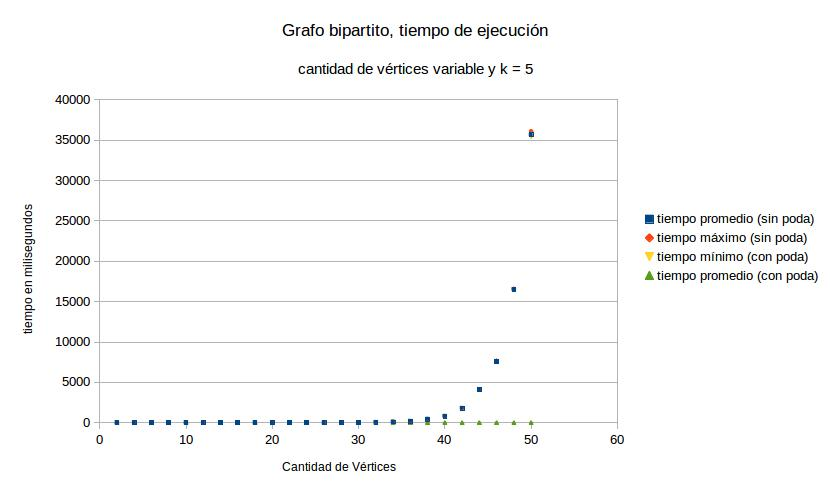
\includegraphics[width=\textwidth,height=3.0in,keepaspectratio
]{bik5.jpg} \newline
\textit{figura 1.a}\newline
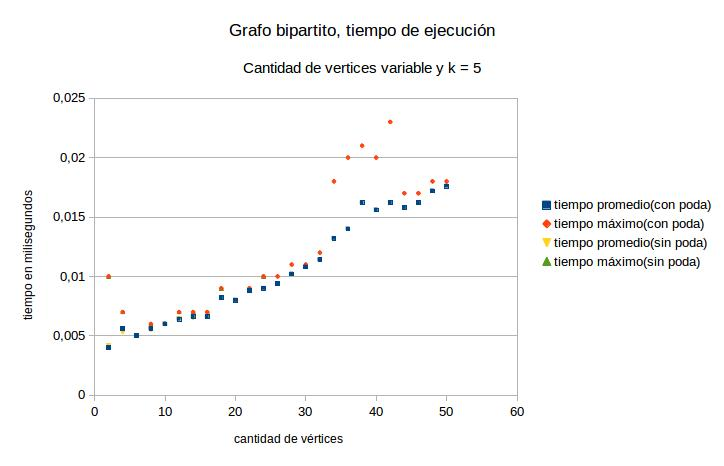
\includegraphics[width=\textwidth,height=3.0in,keepaspectratio
]{kik5se.jpg}\newline
\textit{figura 1.b: Comportamiento de los valores mas chicos de la figura 1.a (ya que la escala establecida en la anterior figura no nos permite apreciar esto)}\newline \newline
Se representa el tiempo de ejecuci\'on estableciendo como variable a la cantidad de v\'ertices y fijando un k, el mismo de valor 5. Al hacer esto la complejidad que hab\'iamos dado seria O($n^{2}*5^{n}$). Como podemos observar es un par\'ametro exponencial por uno polin\'omico. Su representaci\'on deber\'ia asemejarse a una curva. Como es de factor n, mientras crezca el valor de este par\'ametro, mas pronunciado sera el crecimiento de la curva. Lo cual puede observarse en la figura 1.a a partir de aproximadamente el valor 40 la funci\'on empieza a tomar valores cada vez mas altos. Adem\'as comparamos el tiempo de ejecuci\'on para las mismas instancias cuando se utiliza o no la mencionada poda. Como vemos, en aquellos casos en los que se la uso el tiempo de ejecuci\'on es menor. Llegando en algunos casos a haber una notable diferencia, esto se debe a que la cota va a empezar distribuyendo a los v\'ertices entre los conjuntos que se posee. Como estamos en el caso de los bipartitos puede que la distribuci\'on haya sido la \'optima. Y si no lo fue al menos el valor de suma\_solucion es menor que para el caso en el que todos los v\'ertices est\'an dentro del conjunto. Y el total de combinaciones a realizar es menor.  
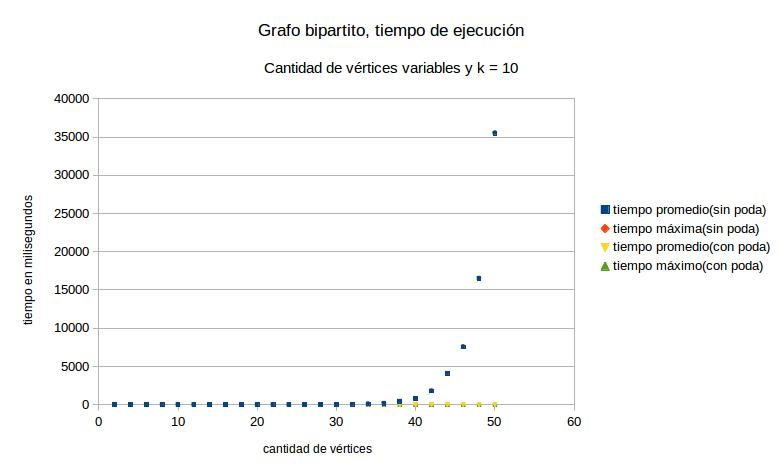
\includegraphics[width=\textwidth,height=3.0in,keepaspectratio
]{bik10.jpg}\newline
\textit{figura 2.a}\newline
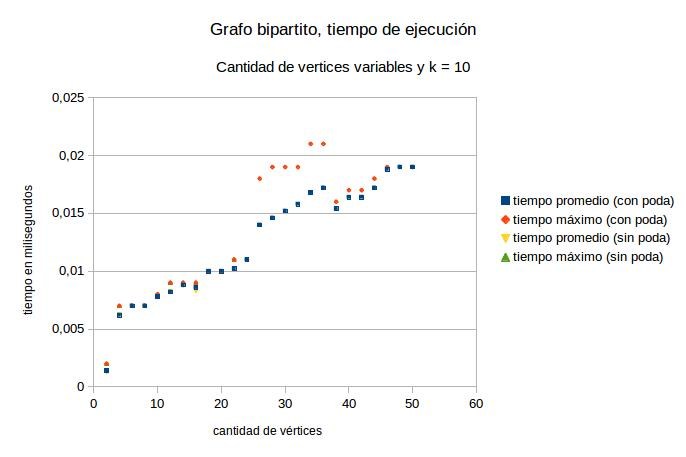
\includegraphics[width=\textwidth,height=3.0in,keepaspectratio
]{bik10seg.jpg} \newline
\textit{figura 2.b:  Comportamiento de los valores mas chicos de la figura 2.a} \newline
A diferencia de la figura anterior para este caso aumentamos el tama\~no de k. Como nuestro algoritmo empieza con un solo conjunto y ve todas las combinaciones posibles para el mismo y luego incrementa la cantidad hasta que haya k conjuntos o $suma\_solucion$ sea igual a cero. Deber\'ia bastar que sin importar la cantidad de conjuntos, sin son mas que dos, el algoritmo finalice luego de agregar al segundo conjunto. Y para mismas instancias de cantidad de v\'ertice el tiempo de ejecuci\'on deber\'ia ser similar. Esto es lo que se observa entre la figura 1 y figura 2. El rango de tiempo de ejecuci\'on en ambos casos es el mismo.  \newline
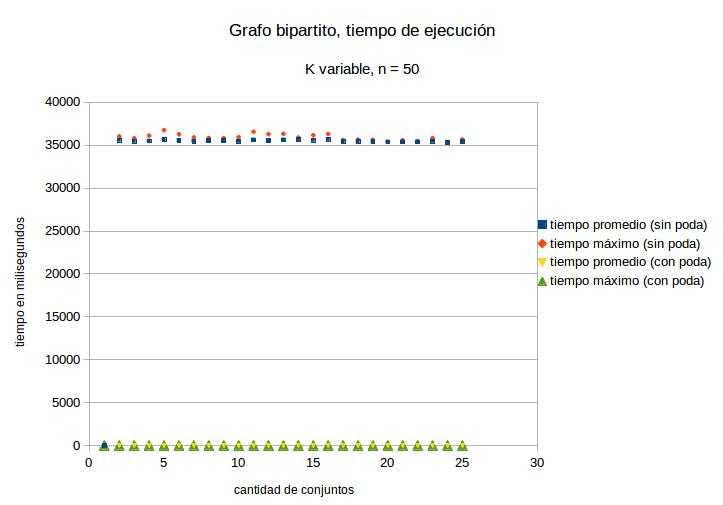
\includegraphics[width=\textwidth,height=3.0in,keepaspectratio
]{bikvar.jpg}\newline
\textit{figura 3}\newline
Para el caso de la $figura$ $3$ se fijo un valor para la cantidad de v\'ertices mientras que el valor de k se modifico en cada instancia. La misma se incremento en uno hasta la cantidad de conjuntos. Como se comento anteriormente, por el funcionamiento del algoritmo, y el tipo de grafo, este termina cuando se ven las combinaciones para un total de dos conjuntos. Entonces sin importar el valor de k (y ahora que n ,cantidad de v\'ertices, esta fijo). Todas las instancias deber\'ian terminar aproximadamente en el mismo tiempo. Y es lo que se observa en este gr\'afico el tiempo de ejecuci\'on se mantiene constante para todos los valores de k. Adem\'as cuando se utiliza la poda, los tiempos de ejecuciones siguen siendo menores.  \newline  
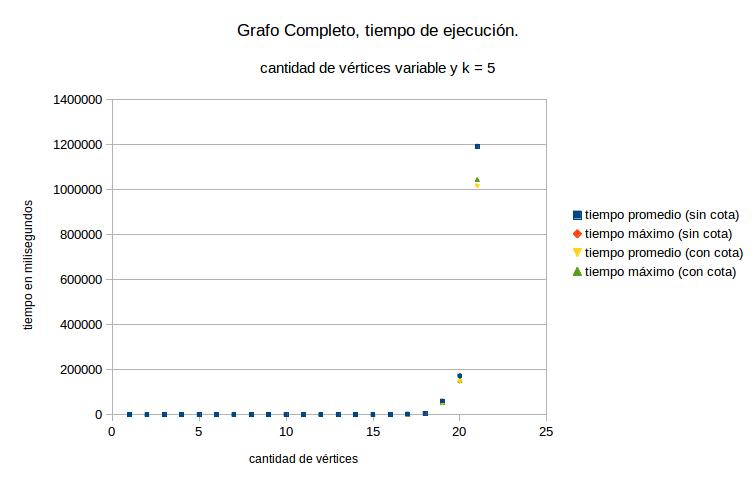
\includegraphics[width=\textwidth,height=3.0in,keepaspectratio
]{complek5.jpg}\newline
\textit{figura 4.a}\newline
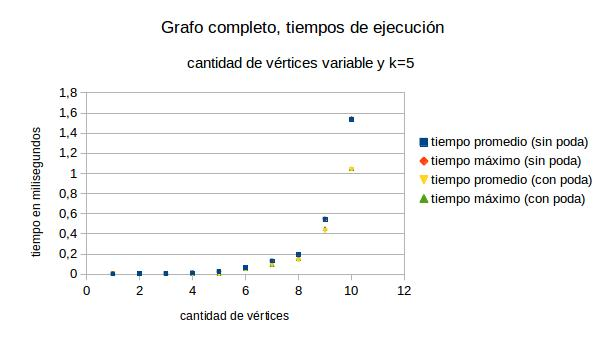
\includegraphics[width=\textwidth,height=3.0in,keepaspectratio
]{comprk5seg.jpg}\newline
\textit{figura 4.b: Comportamiento de los valores mas chicos de la figura 4.a}\newline
En las figuras 4.a y 4.b se observan los tiempos de ejecuci\'on tomando como par\'ametro de entrada un grafo completo. A diferencia de los grafos bipartitos estos terminan para alguna combinacion con los k conjuntos. Ya que al usar mas vamos a tener a menos v\'ertices juntos. Lo cual es favorable ya que ahora todo v\'ertice tiene alg\'un peso con los restantes. En ambas figuras se observa el crecimiento exponencial que tienen los tiempos de ejecuci\'on. Donde a diferencia de los anteriores gr\'aficos el rango de tiempo es mucho mayor. Al usar la poda vemos que no hay una gran mejora. Esto se puede deber a que como ahora estamos trabajando con un completo la distribuci\'on que realiza al comienzo la poda no sirve de mucho, ya que si bien utiliza los k conjuntos. Como ahora todos son adyacentes la distribuci\'on inicial quiz\'as se hizo juntando nodos que suman mucho peso entre ellos. \newline
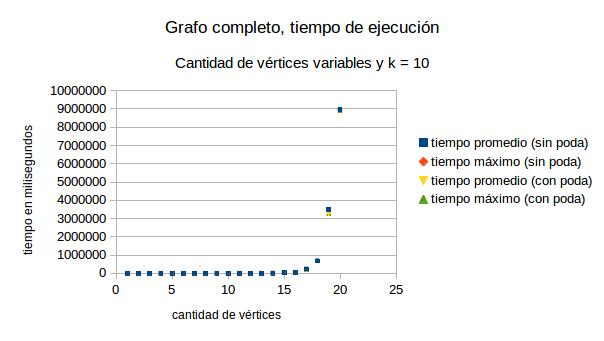
\includegraphics[width=\textwidth,height=3.0in,keepaspectratio
]{comk10.jpg}\newline
\textit{figura 5.a:}\newline
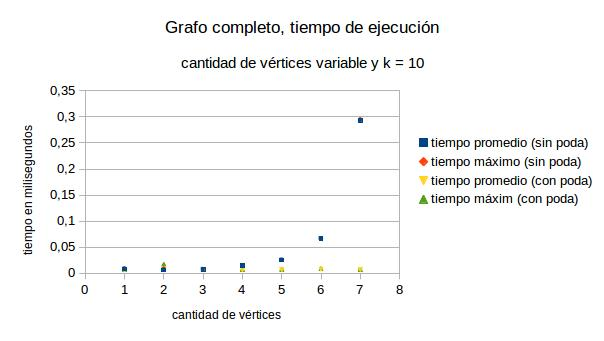
\includegraphics[width=\textwidth,height=3.0in,keepaspectratio
]{comk10seg.jpg}\newline
\textit{figura 5.b:Comportamiento de los valores mas chicos de la figura 5.a}\newline
Para el caso representado en la figura 5.a y 5.b se aumento la cantidad de conjuntos que para el caso de la figuras 4. Por la complejidad que establecimos, si aumentamos el valor de k la complejidad deber\'ia aumentar. Y como pueden observarse en las ultimas figuras esto ocurre. Si bien se utilizan la misma cantidad de v\'ertices que para las figuras 4. El rango de tiempo es mucho mas alto. Y La poda funciona con efectividad para los primeros valores. Sobre todo para los menores a 11 v\'ertice. Ya que la misma habr\'a distribuido a todos los v\'ertices en un conjunto distinto y el peso de eso es cero, finalizando el algoritmo. Sin embargo, para los otros casos solo representa una leve mejora. Ya que establece una cota menor que la de empezar con todos los v\'ertices. Pero aun as\'i se siguen realizando aproximadamente $10^{n}$ combinaciones. \newline
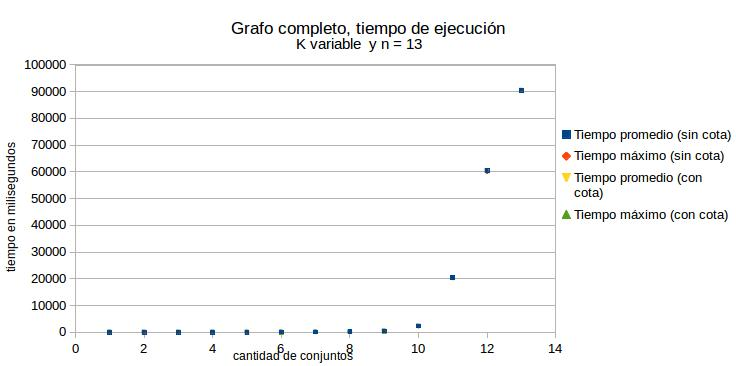
\includegraphics[scale=0.5]{bien.jpg}\newline
\textit{figura 6.a} \newline
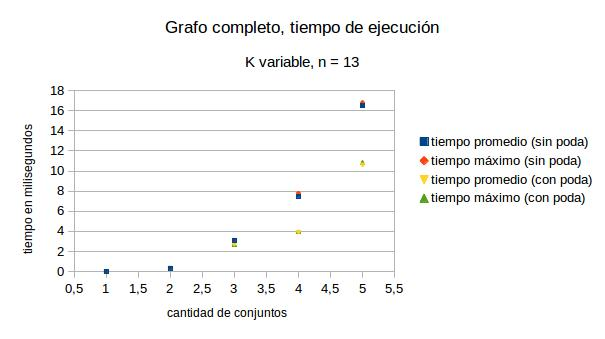
\includegraphics[width=\textwidth,height=3.0in,keepaspectratio
]{comkvarseg.jpg}\newline
\textit{figura 6.b: Comportamiento de los valores mas chicos de la figura 5.a}\newline
En las figuras 6. Se observa el tiempo de ejecuci\'on al establecer un k variable y un n fijo. Si bien hay un crecimiento notable entre los valores de los tiempos de ejecuci\'on, se observa que estos son menos que cuando fij\'abamos un valor para k y n es variable. Por lo que podemos concluir que para obtener tiempos de ejecuciones cortos. Es preferible contar con un valor de k variable y n fijos. Mas aun si estos n no son valores muy grande ya que la complejidad seria solo un valor exponencial, O($k^{c}$), c constante. A diferencia de cuando n es variable que es exponencial por una funci\'on cuadr\'atica, O($n^{2}*k^{n}$).\newline

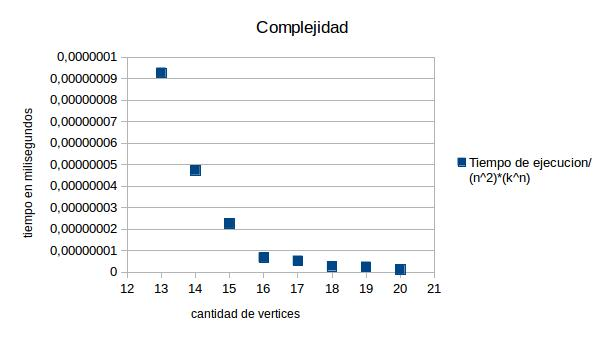
\includegraphics[width=\textwidth,height=3.0in,keepaspectratio
]{comple.jpg}\newline
figura 7: finalmente tratamos de corroborar que nuestra complejidad era la planteada por lo que procedimos a dividir a los tiempos de ejecuci\'on por O($n^{2}*k^{n}$). Si bien al principio se ve que decrece rapidamente. Luego comienza a tender a un mismo n\'umero cuando el valor de n aumenta. Pero debido a que cuando se incrementa el valor de n el tiempo de ejecuci\'on tambien solo podemos corroborar esto para un n\'umero muy acotado. 

\end{document}